% =============================================================================
% sections/design/rover/robotic_arm_mechanical_architecture.tex
% Teams: arm (Marta)
% Status: draft
%
% Scope (per PM): kinematic structure, joint layout, material choices,
% joint-load table. End-effector specs -> critical parts.
%
% Images below are placeholders (teams/arm/figures/arm_photo.png and the
% four manipulator_*.png renders) - swap them for real photos of the built
% arm by overwriting the same files, no need to touch the LaTeX layout.
% Target for arm_photo: built arm with joints q1-q6, machined aluminium
% links, and the quick-change interface labeled; companion idea: dimensioned
% side-view reachability drawing showing the 132 cm reach.
% =============================================================================

\todo[inline]{Verify against the as-built arm: measure actual maximum
reach and confirm the \qty{3}{\kilo\gram} payload at full extension.}

The rover's robotic arm is a 6-DOF articulated manipulator with a maximum
reach of \qty{132}{\centi\meter} and a maximum payload of
\qty{3}{\kilo\gram}: an anthropomorphic RRR positioning group ($q_1$ base
rotation, $q_2$ shoulder pitch, $q_3$ elbow pitch) placing the wrist
center, and a wrist ($q_4$--$q_6$) setting the end-effector
approach angle independently of position, which keeps inverse kinematics
simple and reaches both ground-level sampling targets and elevated
maintenance panels. The assembled arm is pictured in
\autoref{fig:arm_photo}.

The structure is all-aluminium: solid machined shoulder links and
aluminium joint housings throughout, including the wrist. High-torque
planetary actuators drive $q_1$--$q_3$ and compact low-torque units drive
the wrist; a tool-less quick-change interface carries the three
end-effectors, each detailed in its critical-parts section. The
calculated peak joint loads and the resulting actuator safety factors are
summarized in \autoref{tab:joint_loads_actuators}; all motion units carry
dual 14-bit magnetic encoders for closed-loop position feedback.

\begin{table}[htbp]
    \centering
    \caption{Calculated peak joint loads with estimated uncertainty and selected actuator torques}
    \label{tab:joint_loads_actuators}
    \begin{tabular}{lccc}
    \hline
    \textbf{Joint (Coordinate)} &
\makecell{\textbf{Calculated Peak} \\ \textbf{Load [\unit{\newton\metre}]}} &
\makecell{\textbf{Motor Rated} \\ \textbf{Torque [\unit{\newton\metre}]}} &
\makecell{\textbf{Safety} \\ \textbf{Factor}} \\
    \hline
    $q_1, q_2$ (Base, Shoulder) & $44.9 \pm 4.0$  & 48 & 1.07 \\
    $q_3$ (Elbow)               & $16.2 \pm 1.5$  & 48 & 2.96 \\
    $q_4, q_5, q_6$ (Wrist)     & $2.84 \pm 0.30$ & 9  & 3.17 \\
    \hline
    \end{tabular}
\end{table}

\todo[inline]{Loads above are the Preliminary values for the
carbon-tube design — RECALCULATE for the heavier all-aluminium links
(link masses and r-perp changed)}

\begin{figure}[!htbp]
    \centering
    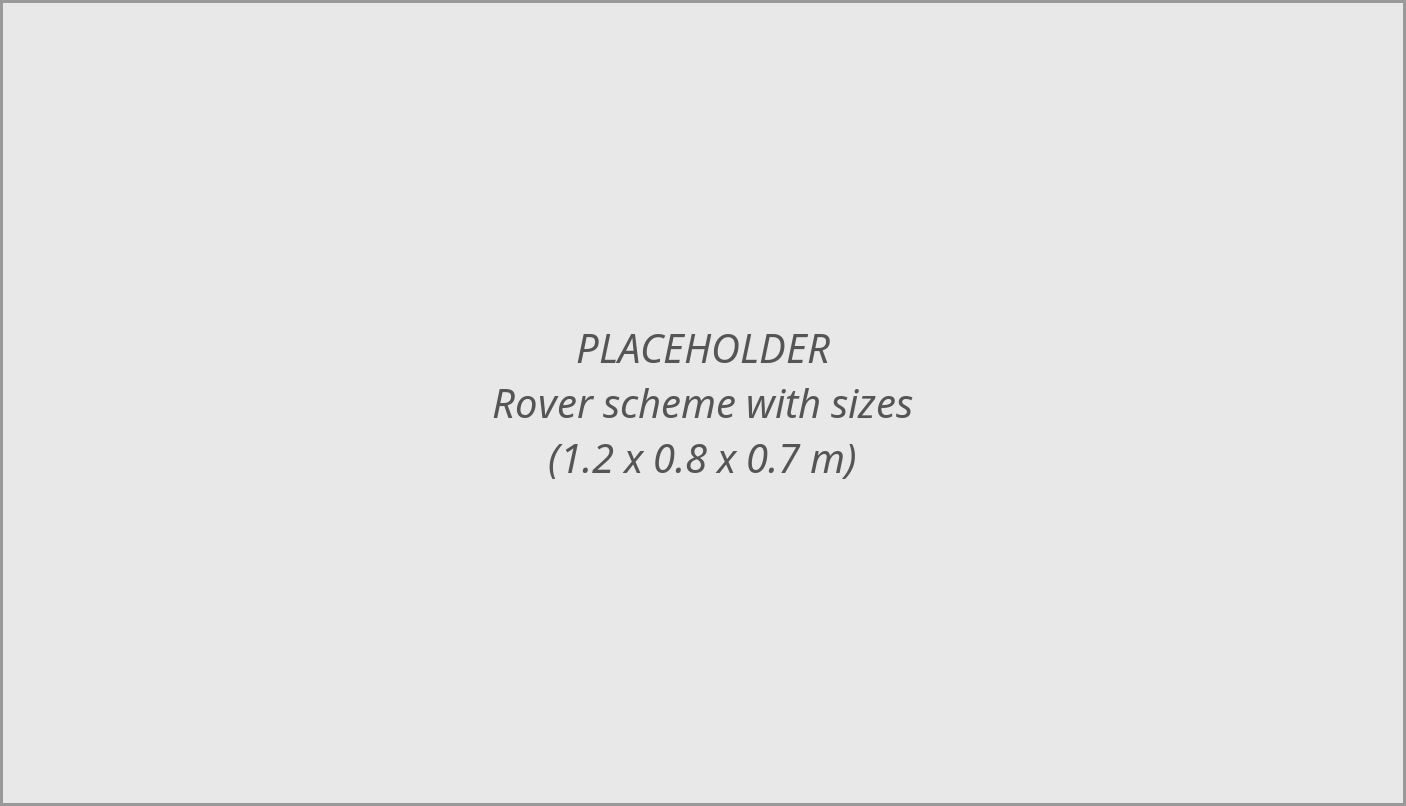
\includegraphics[width=0.8\linewidth]{teams/arm/figures/arm_photo}
    \caption{Indomitus manipulator -- assembled arm with labeled joints
    $q_1$--$q_6$ and quick-change interface}
    \label{fig:arm_photo}
\end{figure}

The manipulator across its four operational scenarios is shown in
\autoref{fig:manipulator_scenarios}.

\begin{figure}[!htbp]
    \centering
    \begin{subfigure}[b]{0.48\textwidth}
        \centering
        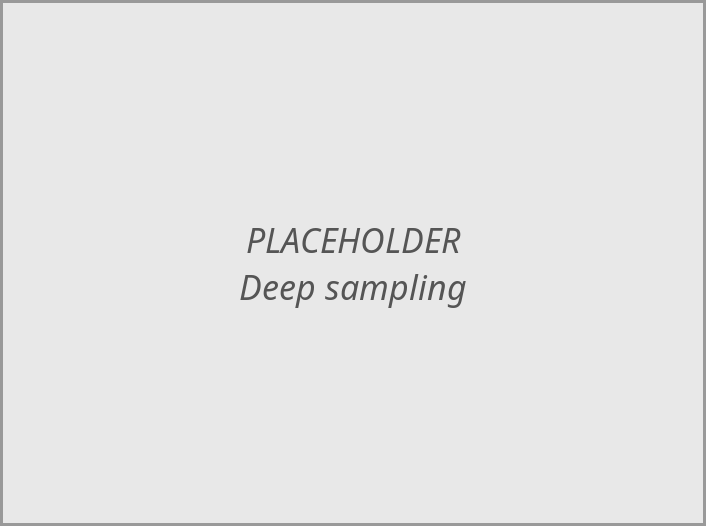
\includegraphics[width=\linewidth]{teams/arm/figures/manipulator_deep_sampling}
        \caption{Deep sampling}
    \end{subfigure}
    \hfill
    \begin{subfigure}[b]{0.48\textwidth}
        \centering
        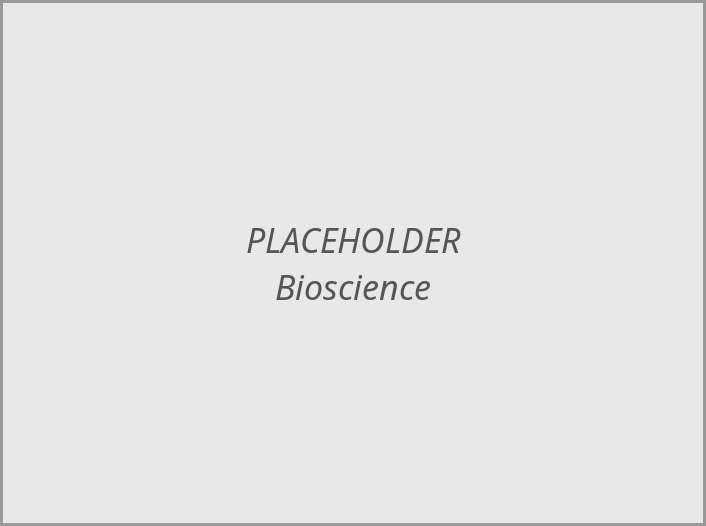
\includegraphics[width=\linewidth]{teams/arm/figures/manipulator_bioscience}
        \caption{Bioscience}
    \end{subfigure}

    \vspace{0.5em}

    \begin{subfigure}[b]{0.48\textwidth}
        \centering
        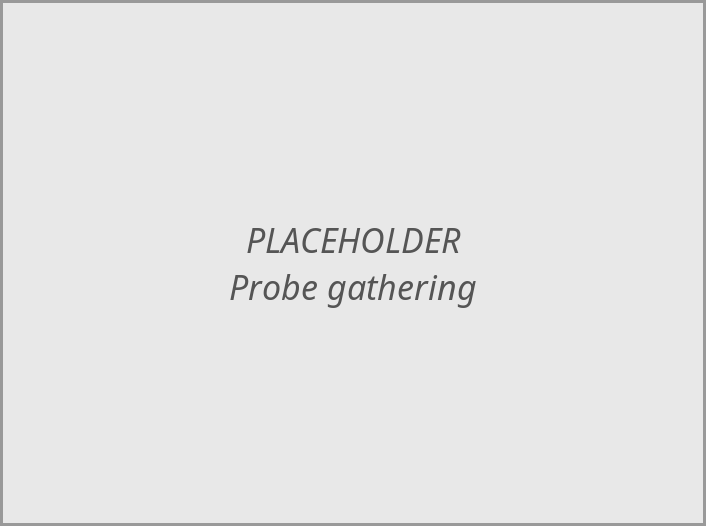
\includegraphics[width=\linewidth]{teams/arm/figures/manipulator_probe_gathering}
        \caption{Probe gathering}
    \end{subfigure}
    \hfill
    \begin{subfigure}[b]{0.48\textwidth}
        \centering
        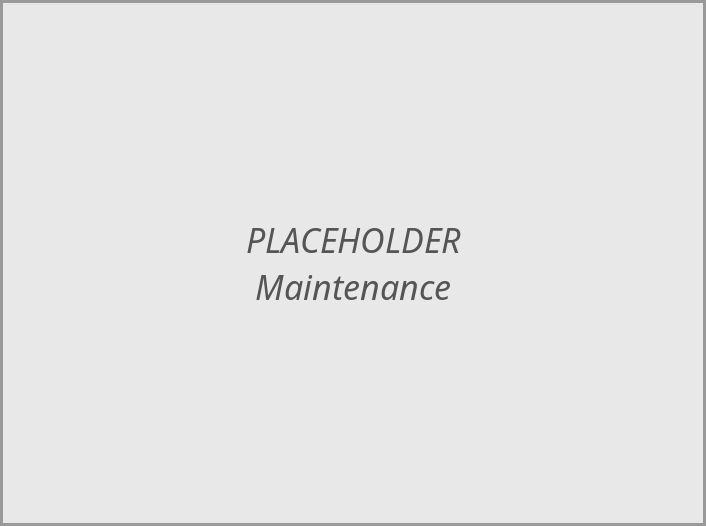
\includegraphics[width=\linewidth]{teams/arm/figures/manipulator_maintenance}
        \caption{Maintenance}
    \end{subfigure}

    \caption{Manipulator configuration and operational scenarios}
    \label{fig:manipulator_scenarios}
\end{figure}